\chapter{Complementary Aspects of the Implementation Phase}
\label{app:annexC}

\section*{Tools and Technologies Used}
This section presents the main tools, libraries, and technologies that supported the development, training, deployment, and visualization throughout the project.

\subsection*{Programming Languages & Environments}
This section presents the primary programming language and development environments used throughout the project. It highlights the flexibility, ease of use, and community support that made these tools essential for building, testing, and managing the overall system.
\subsubsection{Python}

\begin{figure}[H]
    \centering
    \begin{minipage}{0.7\textwidth}
        Python is a versatile and cross-platform programming language, known for its simplicity and efficiency. It supports multiple paradigms and is widely adopted in machine learning and deep learning due to its powerful libraries and active community.
    \end{minipage}%
    \hfill
    \begin{minipage}{0.2\textwidth}
        \centering
        
\includegraphics[width=0.5\linewidth]{appendices/images/Python.png}
    \end{minipage}
\end{figure}




\subsubsection{Google Colab}

\begin{figure}[H]
    \centering
    \begin{minipage}{0.7\textwidth}
        Google Colab is a cloud-based Jupyter Notebook environment that provides free access to \gls{abb:gpu}s and TPUs. It is ideal for machine learning, data analysis, and education, enabling users to write and execute code directly in the browser with minimal setup.
    \end{minipage}%
    \hfill
    \begin{minipage}{0.2\textwidth}
        \centering
        
\includegraphics[width=0.5\linewidth]{appendices/images/GoogleColab.png}
    \end{minipage}
\end{figure}




\subsubsection{Jupyter Notebook}

\begin{figure}[H]
    \centering
    \begin{minipage}{0.7\textwidth}
        Jupyter Notebook and JupyterLab are browser-based tools that combine code, data, and notes in a single workspace. Widely used in data science and research, they offer an organized, customizable environment enhanced by community-built plugins.
    \end{minipage}%
    \hfill
    \begin{minipage}{0.2\textwidth}
        \centering
        
\includegraphics[width=0.5\linewidth]{appendices/images/JupyterNotebook.png}
    \end{minipage}
\end{figure}




\subsubsection{Visual Studio Code}

\begin{figure}[H]
    \centering
    \begin{minipage}{0.7\textwidth}
        Visual Studio Code (VS Code) is a lightweight, open-source editor by Microsoft that supports multiple programming languages. It features code completion, debugging, Git integration, and a wide range of extensions, making it ideal for web and machine learning development.
    \end{minipage}%
    \hfill
    \begin{minipage}{0.2\textwidth}
        \centering
        
\includegraphics[width=0.5\linewidth]{appendices/images/VSCode.png}
    \end{minipage}
\end{figure}



\subsection*{Machine Learning & Deep Learning Libraries}
This section outlines the core libraries and frameworks employed for building and training machine learning and deep learning models. These tools provided efficient implementations of algorithms and architectures required for classification, detection, and model evaluation tasks.

\subsubsection{TensorFlow}

\begin{figure}[H]
    \centering
    \begin{minipage}{0.7\textwidth}
TensorFlow is an open-source machine learning library developed by Google. It serves as a powerful toolkit for solving highly complex mathematical problems with ease. It enables researchers to design experimental architectures and turn them into deployable software solutions.

    \end{minipage}%
    \hfill
    \begin{minipage}{0.2\textwidth}
        \centering
        
\includegraphics[width=0.5\linewidth]{appendices/images/TensorFlow.png}
    \end{minipage}
\end{figure}


% \subsubsection{Keras}

% \begin{figure}[H]
%     \centering
%     \begin{minipage}{0.8\textwidth}
% Keras is an open-source library with fast integration between loss, activation, and optimization functions that are used in machine learning. It can be used with both CNN and RNN. Keras is a part of the TensorFlow 2 Ecosystem, which spans from data handling, modelling, training, hyperparameter tuning, and deployment solutions.

%     \end{minipage}%
%     \hfill
%     \begin{minipage}{0.2\textwidth}
%         \centering
%         
\includegraphics[width=0.5\linewidth]{appendices/images/Keras.png}
%     \end{minipage}
% \end{figure}


\subsubsection{PyTorch }

\begin{figure}[H]
    \centering
    \begin{minipage}{0.7\textwidth}
        TensorFlow is an open-source machine learning library developed by Google. It provides a comprehensive framework for building and deploying machine learning and deep learning models, making it a popular choice among researchers and developers.
    \end{minipage}%
    \hfill
    \begin{minipage}{0.2\textwidth}
        \centering
        
\includegraphics[width=0.5\linewidth]{appendices/images/PyTorch.png}
    \end{minipage}
\end{figure}


\subsubsection{Ultralytics }

\begin{figure}[H]
    \centering
    \begin{minipage}{0.7\textwidth}
        Ultralytics offers YOLO models, such as YOLOv8, for fast and accurate object detection. These models are ideal for real-time tasks like surveillance and robotics and can be easily used with just a few lines of Python code.
    \end{minipage}%
    \hfill
    \begin{minipage}{0.2\textwidth}
        \centering
        
\includegraphics[width=0.5\linewidth]{appendices/images/Ultralytics.png}
    \end{minipage}
\end{figure}


\subsubsection{scikit-learn}

\begin{figure}[H]
    \centering
    \begin{minipage}{0.7\textwidth}
        Scikit-learn is a Python library that simplifies machine learning tasks like classification, regression, and clustering. With built-in algorithms, datasets, and preprocessing tools, it offers a clean and consistent API ideal for data analysis and predictive modeling.
    \end{minipage}%
    \hfill
    \begin{minipage}{0.2\textwidth}
        \centering
        
\includegraphics[width=0.5\linewidth]{appendices/images/scikit-learn.png}
    \end{minipage}
\end{figure}




% \subsubsection{Imbalanced-learn}

% \begin{figure}[H]
%     \centering
%     \begin{minipage}{0.8\textwidth}
% Imbalanced-learn (imblearn) is a Python library that handles class imbalance in machine learning datasets. It provides resampling techniques (oversampling, undersampling, SMOTE) and ensemble methods to improve model performance on imbalanced data. Seamlessly integrates with scikit-learn for easy workflow integration. Essential for fraud detection, medical diagnosis & other imbalance-sensitive tasks.
%     \end{minipage}%
%     \hfill
%     \begin{minipage}{0.2\textwidth}
%         \centering
%         
\includegraphics[width=0.5\linewidth]{appendices/images/Imbalanced-learn.png}
%     \end{minipage}
% \end{figure}


\subsubsection{Joblib}

\begin{figure}[H]
    \centering
    \begin{minipage}{0.7\textwidth}
        Joblib is a Python library designed for efficient saving and loading of machine learning models with large NumPy arrays. It supports parallel processing and memory caching, making it well-suited for scikit-learn workflows and large-scale ML pipelines.
    \end{minipage}%
    \hfill
    \begin{minipage}{0.2\textwidth}
        \centering
        
\includegraphics[width=0.5\linewidth]{appendices/images/Joblib.png}
    \end{minipage}
\end{figure}



\subsection*{Data Handling & Processing}
Efficient data handling is critical in any machine learning pipeline. This section covers the tools used for data manipulation, preprocessing, and transformation essential steps ensuring high-quality model training and evaluation inputs.


\subsubsection{NumPy}

\begin{figure}[H]
    \centering
    \begin{minipage}{0.7\textwidth}
        NumPy is a fundamental Python library for numerical computing, offering efficient multi-dimensional arrays and fast mathematical operations. It is widely used in data science, machine learning, and deep learning as the backbone for libraries like Pandas, scikit-learn, and TensorFlow.
    \end{minipage}%
    \hfill
    \begin{minipage}{0.2\textwidth}
        \centering
        
\includegraphics[width=0.5\linewidth]{appendices/images/NumPy.png}
    \end{minipage}
\end{figure}



\subsubsection{OpenCV}

\begin{figure}[H]
    \centering
    \begin{minipage}{0.7\textwidth}
        OpenCV is an open-source library for computer vision and image processing. It offers optimized algorithms for tasks like object detection, face recognition, and motion tracking, with support for multiple languages and platforms.
    \end{minipage}%
    \hfill
    \begin{minipage}{0.2\textwidth}
        \centering
        
\includegraphics[width=0.5\linewidth]{appendices/images/OpenCV.png}
    \end{minipage}
\end{figure}



\subsubsection{Albumentations}

\begin{figure}[H]
    \centering
    \begin{minipage}{0.7\textwidth}
        Albumentations is a fast and flexible image augmentation library for computer vision. It offers a wide range of high-quality transformations and integrates easily with PyTorch and TensorFlow, making it ideal for improving model performance and robustness.
    \end{minipage}%
    \hfill
    \begin{minipage}{0.2\textwidth}
        \centering
        
\includegraphics[width=0.5\linewidth]{appendices/images/Albumentations.png}
    \end{minipage}
\end{figure}





% \subsubsection{Pillow}

% Pillow is a friendly and easy-to-use Python imaging library, which is a modern fork of the original PIL (Python Imaging Library). It supports opening, manipulating, and saving many different image file formats. Pillow is commonly used for basic image processing tasks such as resizing, cropping, rotating, filtering, and converting image formats in machine learning and web applications.


\subsection*{Visualization Libraries}

Visual analysis plays a key role in understanding data behavior and model performance. This section includes the libraries used for plotting, graphing, and visually representing both datasets and model metrics in an informative way.

\subsubsection{Matplotlib}

\begin{figure}[H]
    \centering
    \begin{minipage}{0.7\textwidth}
        Matplotlib is a popular Python library for creating static and interactive visualizations. It supports various plot types like line charts, histograms, and scatter plots, making it essential for data analysis and model evaluation.
    \end{minipage}%
    \hfill
    \begin{minipage}{0.2\textwidth}
        \centering
        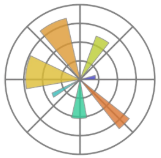
\includegraphics[width=0.5\linewidth]{appendices/images/Matplotlib.png}
    \end{minipage}
\end{figure}



\subsubsection{Seaborn}

\begin{figure}[H]
    \centering
    \begin{minipage}{0.7\textwidth}
        Seaborn is a Python visualization library based on Matplotlib, designed for creating attractive and informative statistical plots. It simplifies complex visualizations like heatmaps and box plots, making it a valuable tool for data analysis and machine learning.
    \end{minipage}%
    \hfill
    \begin{minipage}{0.2\textwidth}
        \centering
        
\includegraphics[width=0.5\linewidth]{appendices/images/Seaborn.png}
    \end{minipage}
\end{figure}



\subsection*{Annotation & Dataset Preparation}
Accurate labeling and proper dataset structuring are foundational to supervised learning. This section presents the tools used for annotating images and organizing datasets, supporting tasks such as object detection and classification.


\subsubsection{Computer Vision Annotation Tool (CVAT)}

\begin{figure}[H]
    \centering
    \begin{minipage}{0.7\textwidth}
        CVAT (Computer Vision Annotation Tool) is an open-source web tool by Intel for annotating images and videos. It supports bounding boxes, polygons, and masks, making it ideal for creating high-quality datasets for object detection, segmentation, and tracking.
    \end{minipage}%
    \hfill
    \begin{minipage}{0.2\textwidth}
        \centering
        
\includegraphics[width=0.5\linewidth]{appendices/images/CVAT.png}
    \end{minipage}
\end{figure}



\subsection*{Visual Design}
Visual design was essential for planning and presenting the system. This section covers tools used to create \gls{abb:ui} mockups and system diagrams, aiding in workflow visualization and user experience design.


\subsubsection{Lucidchart}

\begin{figure}[H]
    \centering
    \begin{minipage}{0.7\textwidth}
        Lucidchart is a web-based tool for creating diagrams and flowcharts. Accessible from any browser, it supports a wide range of visualizations including UML diagrams, wireframes, mind maps, and network diagrams, making it ideal for collaboration and project planning.
    \end{minipage}%
    \hfill
    \begin{minipage}{0.2\textwidth}
        \centering
        
\includegraphics[width=0.5\linewidth]{appendices/images/Lucidchart.png}
    \end{minipage}
\end{figure}




\subsubsection{Figma}

\begin{figure}[H]
    \centering
    \begin{minipage}{0.7\textwidth}
        Figma is a cloud-based tool for designing user interfaces, wireframes, and prototypes. It supports real-time collaboration and is widely used for web and mobile design, offering a smooth workflow from design to development.
    \end{minipage}%
    \hfill
    \begin{minipage}{0.2\textwidth}
        \centering
        
\includegraphics[width=0.5\linewidth]{appendices/images/Figma.png}
    \end{minipage}
\end{figure}



\subsection*{Web Development & Deployment}
This section introduces the tools and technologies used to develop and deploy the web-based components of the project. It includes front-end and back-end frameworks, as well as platforms for API integration, testing, and final deployment of the application.

\subsubsection{Flask}

\begin{figure}[H]
    \centering
    \begin{minipage}{0.7\textwidth}
        Flask is a lightweight Python web framework used to build web applications and APIs. Its simplicity and flexibility make it ideal for integrating machine learning models and deploying data-driven solutions.
    \end{minipage}%
    \hfill
    \begin{minipage}{0.2\textwidth}
        \centering
        
\includegraphics[width=0.5\linewidth]{appendices/images/Flask.png}
    \end{minipage}
\end{figure}


\subsubsection{React}

\begin{figure}[H]
    \centering
    \begin{minipage}{0.7\textwidth}
        React is an open-source JavaScript library developed by Meta for building dynamic and responsive user interfaces. It enables the creation of reusable components and is commonly used for single-page applications (SPAs).
    \end{minipage}%
    \hfill
    \begin{minipage}{0.2\textwidth}
        \centering
        
\includegraphics[width=0.5\linewidth]{appendices/images/React.png}
    \end{minipage}
\end{figure}


\subsubsection{Tailwind CSS}

\begin{figure}[H]
    \centering
    \begin{minipage}{0.7\textwidth}
        Tailwind CSS is a utility-first framework that allows rapid and responsive \gls{abb:ui} development using pre-defined classes. It streamlines styling directly in \gls{abb:html} or JSX, offering flexibility and consistency without writing custom CSS.
    \end{minipage}%
    \hfill
    \begin{minipage}{0.2\textwidth}
        \centering
        
\includegraphics[width=0.5\linewidth]{appendices/images/TailwindCSS.png}
    \end{minipage}
\end{figure}



\subsubsection{Vite}

\begin{figure}[H]
    \centering
    \begin{minipage}{0.7\textwidth}
        Vite is a fast front-end build tool that offers instant server start, efficient hot module replacement, and optimized production builds. It is commonly used with frameworks like React and tools like Tailwind CSS to enhance development speed and performance.
    \end{minipage}%
    \hfill
    \begin{minipage}{0.2\textwidth}
        \centering
        
\includegraphics[width=0.5\linewidth]{appendices/images/Vite.png}
    \end{minipage}
\end{figure}




\section*{Extended Web Platform Pages}

\subsection*{Home page}
The Home Page of Wheat Guard introduces our AI-powered platform for monitoring wheat crop health. The top navigation bar provides quick access to About the App, Services, Docs, Chatbot, and Contact Us. A welcoming message and a Get Started button encourage users to explore the platform easily.
\begin{figure}[H]
    \centering
    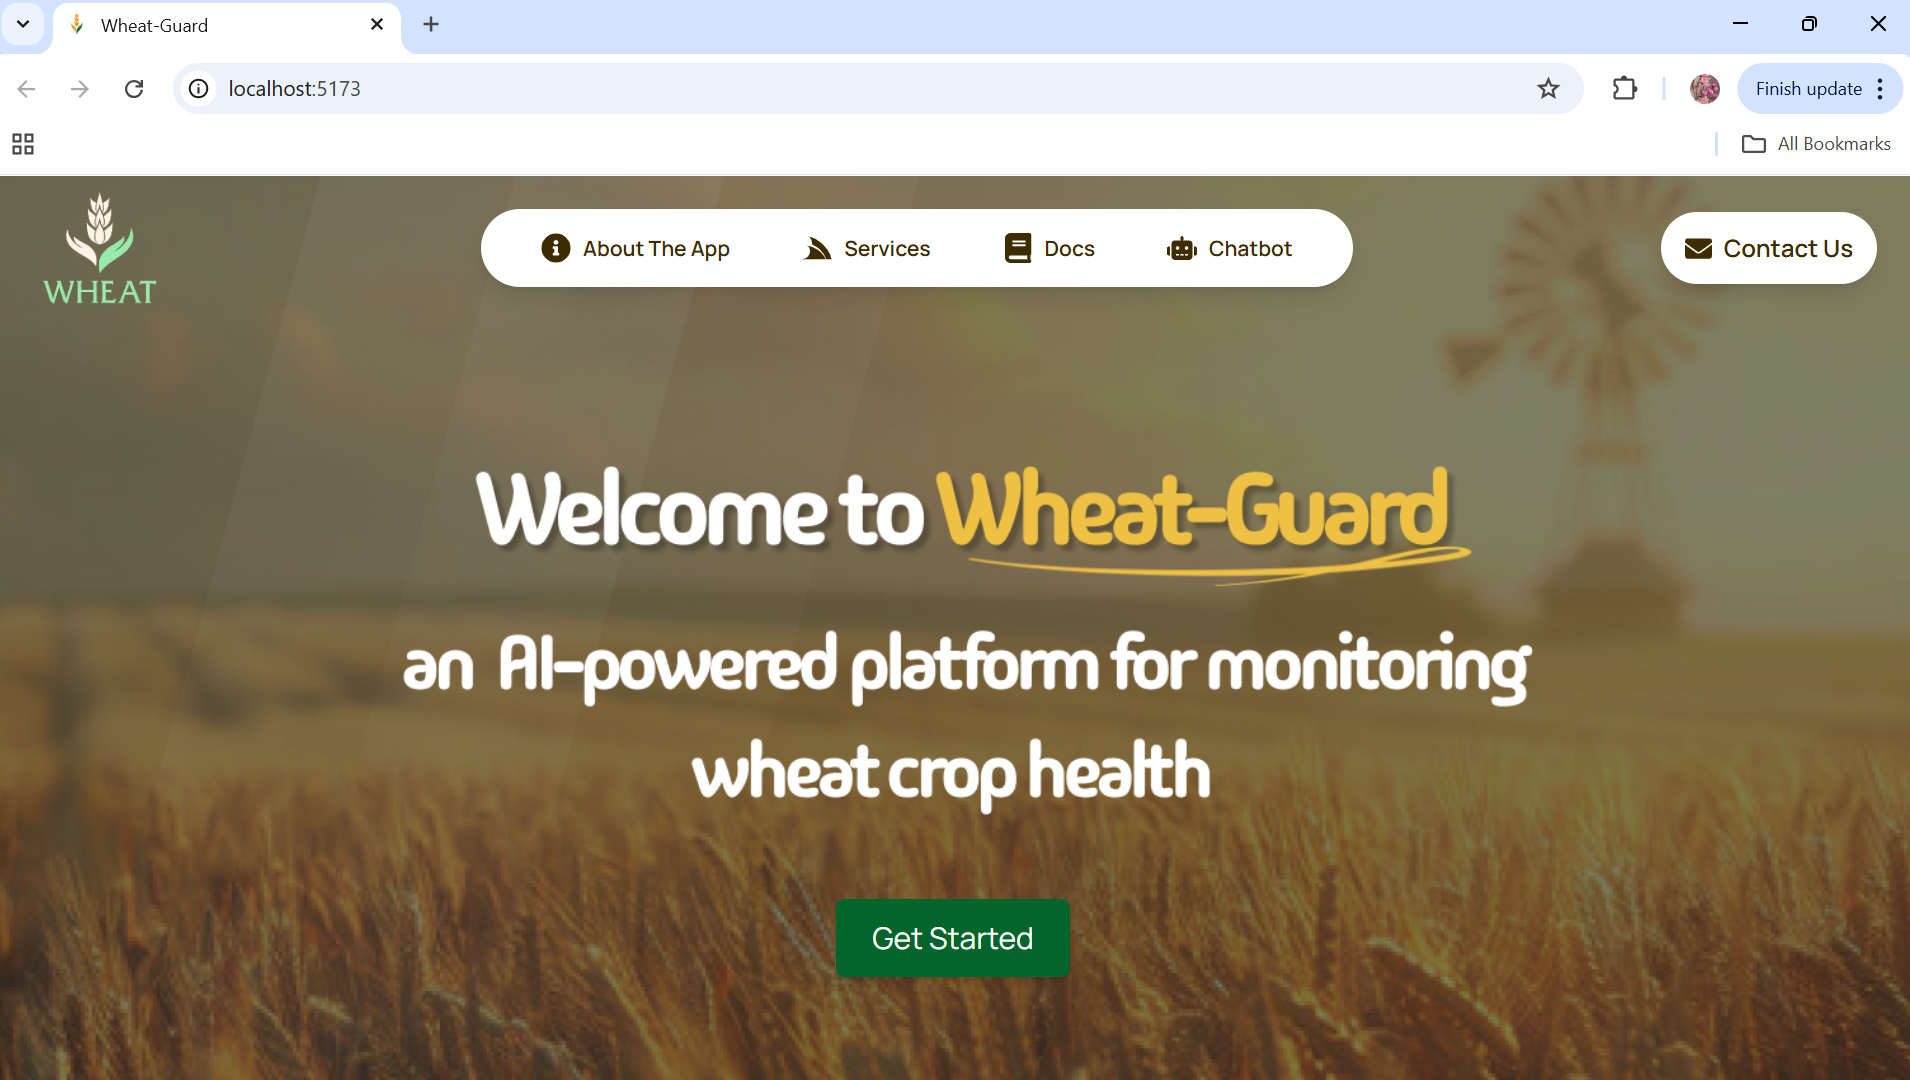
\includegraphics[width=0.6
    \textwidth]{appendices/images/HomePage.png}
    \caption{Home Page \protect\parencite{fang2023lightweight}.}
    \label{fig:HomePage}
\end{figure}



\subsection*{About page}
The About Page of Wheat-Guard highlights the mission of empowering farmers with AI-driven technology to monitor, detect, and optimize wheat crop health. It emphasizes accurate, early disease detection to help maximize yields and reduce losses, supported by visuals and a Discover More button for deeper exploration.

% \begin{figure}[H]
%     \centering
%     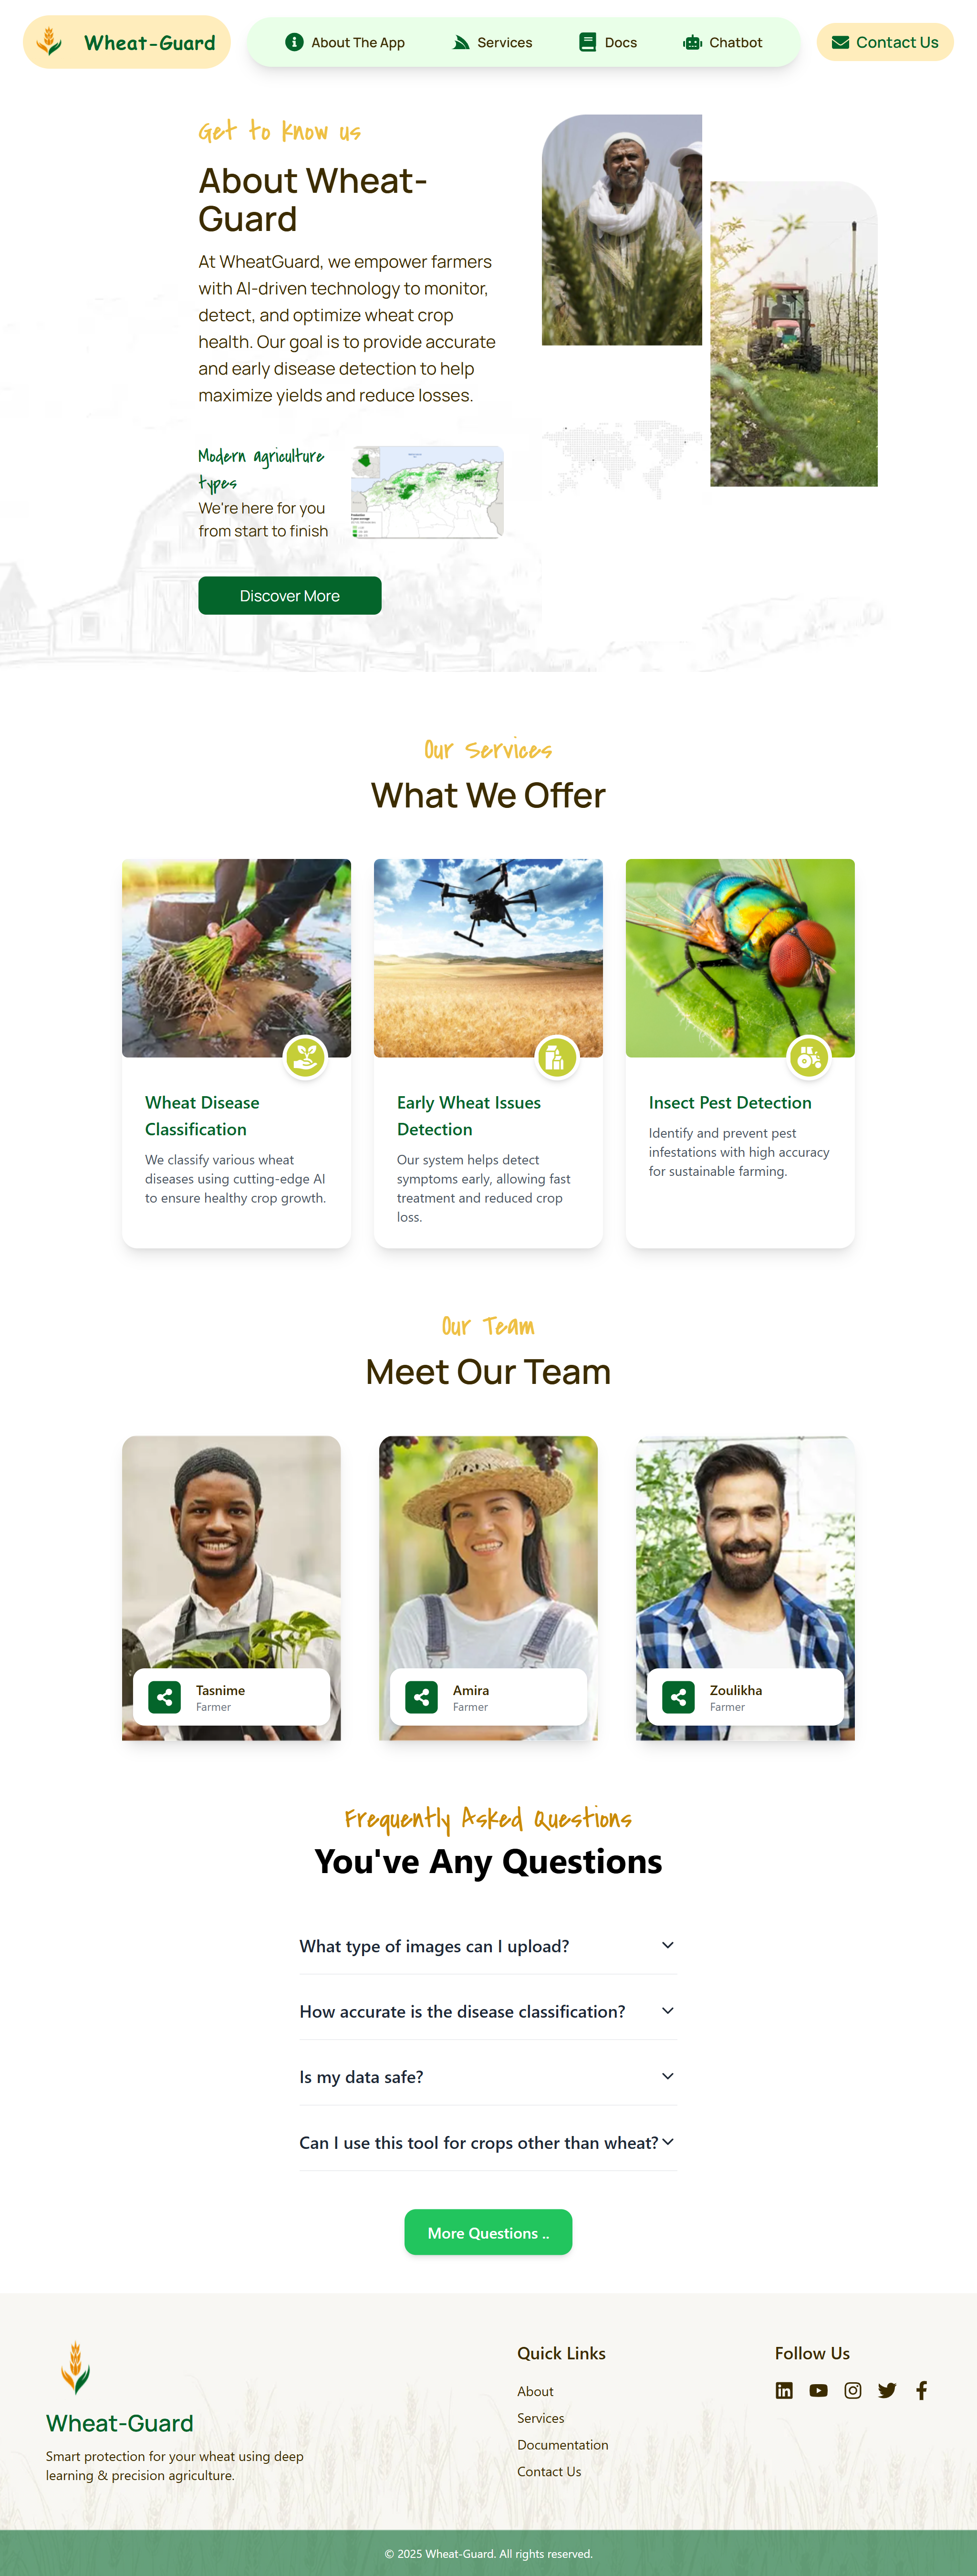
\includegraphics[width=0.5
%     \textwidth]{appendices/images/About.png}
%     \caption{Home Page.}
%     \label{fig:About}
% \end{figure}

\subsection*{Documentation page}
This page introduces Wheat-Guard's key features, including AI-powered disease detection, early crop issue monitoring, pest identification, and actionable farming insights. It provides a quick overview to help users understand the app’s core functionalities and how it supports healthier wheat farming.


% \begin{figure}[H]
%     \centering
%     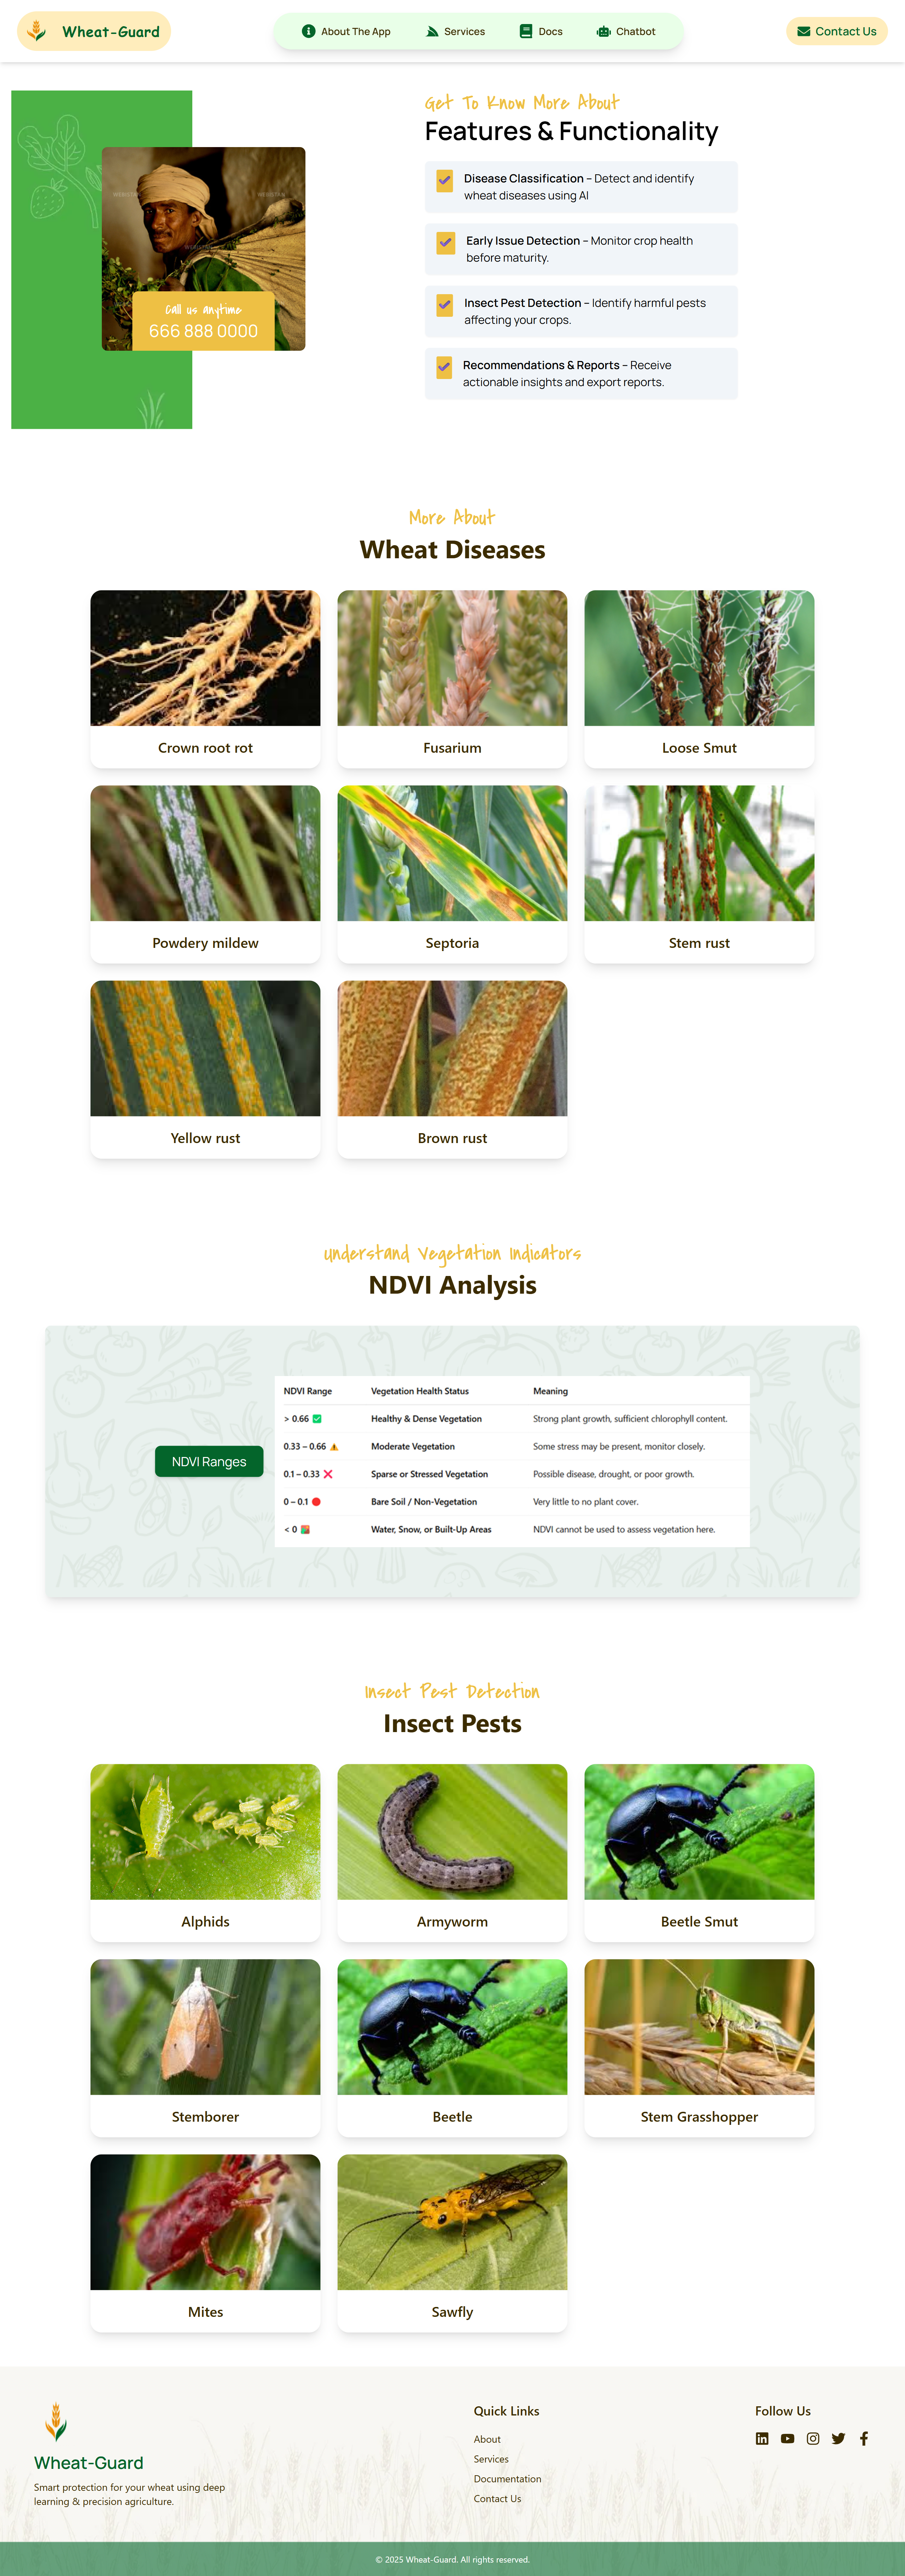
\includegraphics[width=0.5
%     \textwidth]{appendices/images/Documentation.png}
%     \caption{Documentation Page.}
%     \label{fig:Documentation}
% \end{figure}

\begin{figure}[H]
    \centering
    \begin{minipage}{0.48\textwidth}
        \centering
        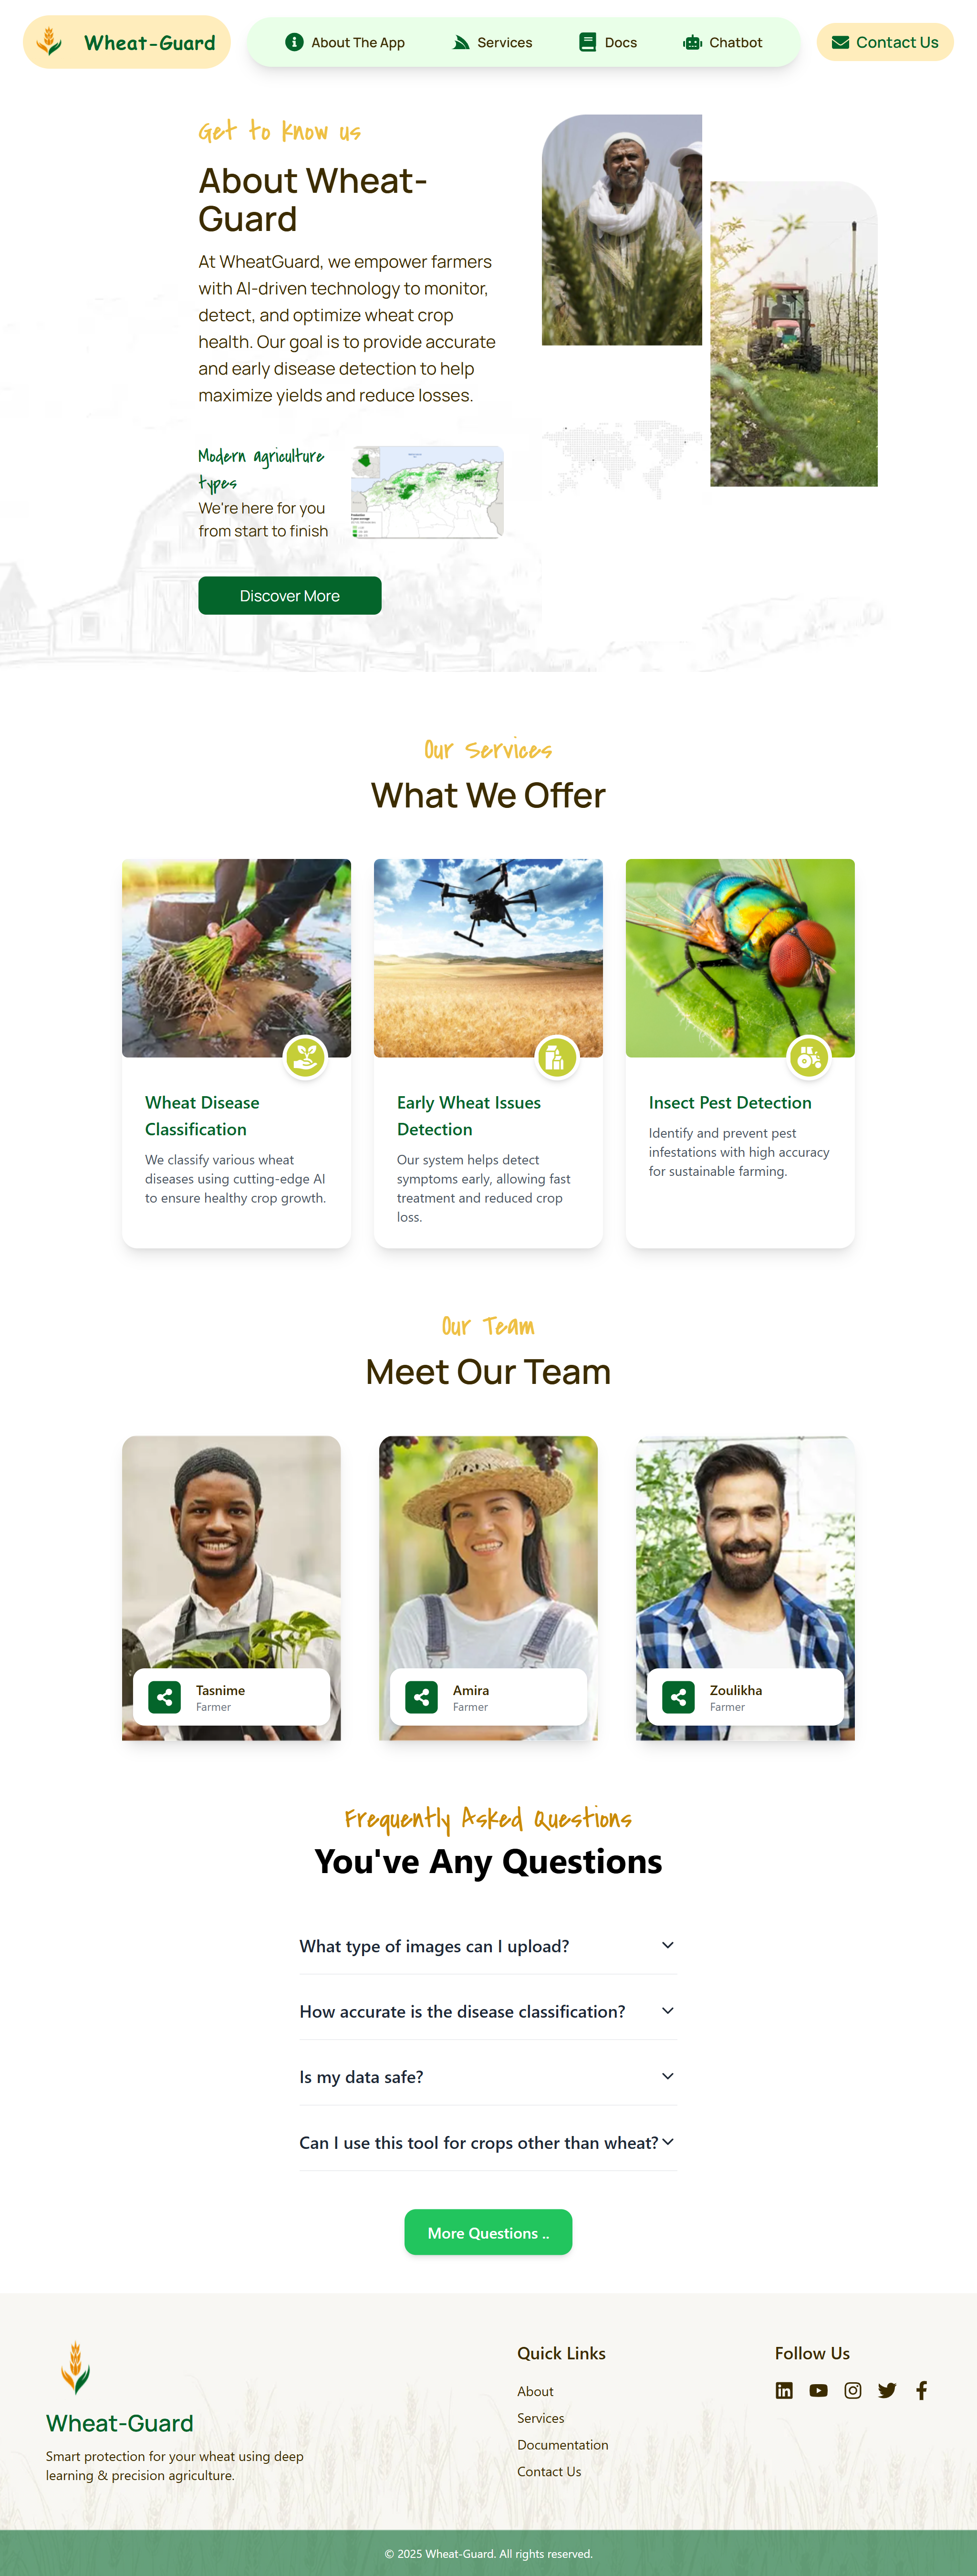
\includegraphics[width=\linewidth]{appendices/images/About.png}
        \caption{Home Page.}
        \label{fig:About}
    \end{minipage}
    \hfill
    \begin{minipage}{0.48\textwidth}
        \centering
        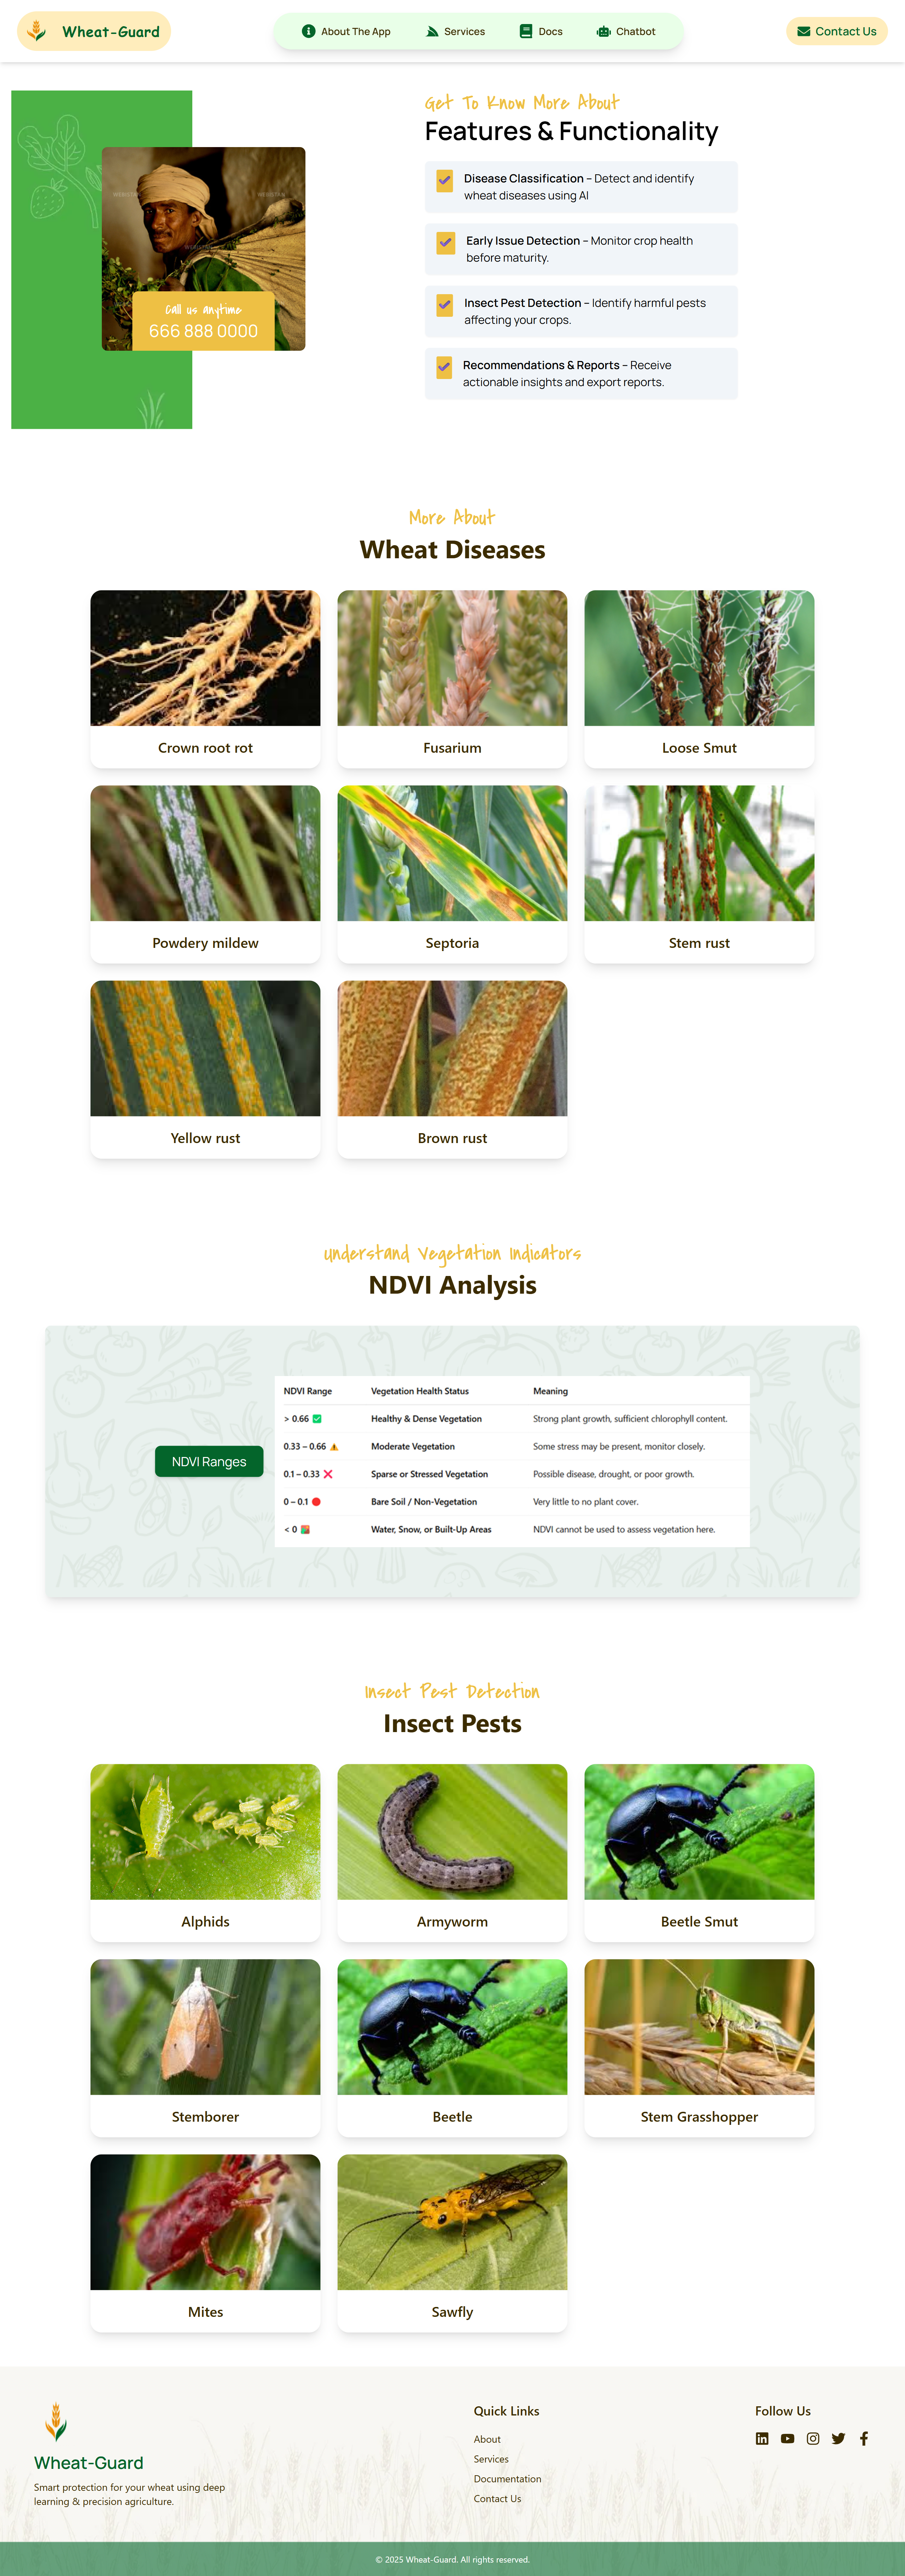
\includegraphics[width=\linewidth]{appendices/images/Documentation.png}
        \caption{Documentation Page.}
        \label{fig:Documentation}
    \end{minipage}
\end{figure}



\subsection*{Contact page}
This page provides all the ways to get in touch with the Wheat-Guard team. Use it for technical support, questions about the app, or to share feedback and suggestions.
\begin{figure}[H]
    \centering
    
\includegraphics[width=0.6
    \textwidth]{appendices/images/ContactUs.png}
    \caption{Contact Page.}
    \label{fig:Contact}
\end{figure}






